%\documentclass[tikz,border=5pt]{standalone}
\begin{document}
	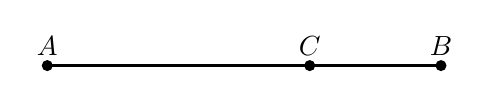
\begin{tikzpicture}
		% 绘制5cm长的线段AB
		\draw[line width=1pt] (0,0) -- (5cm,0);
		% 标记点A、B、C
		\fill (0,0) circle (2pt) node[above] {$A$};                % 点A(起点)
		\fill (5cm,0) circle (2pt) node[above] {$B$};              % 点B(终点)
		\fill (5cm - 5cm/3,0) circle (2pt) node[above] {$C$};      % 点C(距B点1/3处)
	\end{tikzpicture}
\end{document}
